\section{EMPIRICAL ANALYSIS}

\subsection{Explaining Differences in Job Tasks}

\begin{onehalfspace}
This section analyzes the degree to which the tasks performed by workers
within their respective jobs can be explained by factors such as their
human capital, demographic characteristics, and the technical requirements
intrinsic to the job itself. These technical requirements are approximated
through the utilization of detailed occupation dummies. Our analytical
approach is based on descriptive Ordinary Least Squares (OLS) regressions,
which are structured as follows
\begin{equation}
T_{ij}=\alpha+\delta_{1}C_{i}+\delta_{2}\mathbf{X_{i}}+\gamma_{j}+\lambda_{i}+\varepsilon_{ij}\label{eq:descriptive_ols}
\end{equation}

Where the vector of $C$ denotes the human capital measures (education,
computer experience, job experience), vector $\mathbf{X}$, denotes
the demographic variables (parents' educational attainment, age and
gender), $\gamma$ is a vector of 2-digit occupation dummies and $\lambda$
denotes the vector of firm size (3 categories) and industry (21 categories
in total) dummies. The reference group is a female with lower secondary
or less education between the ages of 15-19, whose parents have not
completed upper secondary school. The results of the estimation are
presented in Table \ref{tab:Estimation-Results-of-tasks}.

Table \ref{tab:Estimation-Results-of-tasks} shows significant associations
with some variables. The even-numbered columns (2, 4 and 6) correspond
to estimations with 2-digit ISCO08 occupation dummies. Including occupation
dummies induces a substantial augmentation in the model's fit across
all task categories. Notably, when the occupation dummies are included,
the explanatory power reaches 35.5\% for the abstract tasks. Furthermore,
the education dummies are statistically significant for most of the
regressions and their coefficients are increasing (in absolute terms)
with more years spent in school. While the coefficients of education
dummies are positive for abstract task scores, for the other two task
categories, it takes negative values, indicating a notable positive
correlation between abstract tasks and skills acquired during formal
education, as the coefficient's magnitude increases with the years
spent in school. Notably, the coefficients of education dummies are
decreased in all the task categories, when we control for the occupation
dummies. This observation indicates that the relationship between
education and task categories depends on the occupational assignment.
In particular, concerning manual tasks, introducing occupational dummies
leads to the loss of significance in the association between educational
attainment and manual tasks. Males lower use of abstract tasks persists
with the occupation controls, but this is not the case for routine
tasks. The occupational assignment primarily mediates the significance
of the positive relationship.
\end{onehalfspace}
\begin{center}
\begin{table}[H]
\caption{\label{tab:Estimation-Results-of-tasks}Estimation Results of Task
Scores with Individual Characteristics}

\begin{centering}
\noindent\resizebox{\textwidth}{!}{%
\begin{tabular}{lllllll}
\toprule 
 & \multicolumn{2}{l}{Abstract} & \multicolumn{2}{l}{Routine} & \multicolumn{2}{l}{Manual}\tabularnewline
\cmidrule{2-7} \cmidrule{3-7} \cmidrule{4-7} \cmidrule{5-7} \cmidrule{6-7} \cmidrule{7-7} 
 & (1) & (2) & (3) & (4) & (5) & (6)\tabularnewline
\cmidrule{2-7} \cmidrule{3-7} \cmidrule{4-7} \cmidrule{5-7} \cmidrule{6-7} \cmidrule{7-7} 
\textbf{Human Capital} &  &  &  &  &  & \tabularnewline
\multicolumn{7}{l}{\textit{Education dummy (base=lower secondary or less)}}\tabularnewline
Upper secondary & 0.23$^{***}$ & 0.13$^{*}$ & -0.13$^{*}$ & -0.04 & -0.10 & 0.05\tabularnewline
 & (0.06) & (0.05) & (0.06) & (0.06) & (0.06) & (0.06)\tabularnewline
Tertiary 2-3 years & 0.70$^{***}$ & 0.50$^{***}$ & -0.51$^{***}$ & -0.30$^{***}$ & -0.18 & 0.06\tabularnewline
 & (0.09) & (0.09) & (0.09) & (0.09) & (0.10) & (0.09)\tabularnewline
Tertiary 4 years & 1.05$^{***}$ & 0.68$^{***}$ & -0.78$^{***}$ & -0.39$^{***}$ & -0.35$^{***}$ & -0.06\tabularnewline
 & (0.08) & (0.09) & (0.08) & (0.10) & (0.09) & (0.10)\tabularnewline
Tertiary Master & 1.39$^{***}$ & 0.96$^{***}$ & -1.10$^{***}$ & -0.63$^{***}$ & -0.58$^{***}$ & -0.24\tabularnewline
 & (0.15) & (0.15) & (0.15) & (0.16) & (0.16) & (0.16)\tabularnewline
No computer exp. & -0.30$^{***}$ & -0.20 & 0.40$^{***}$ & 0.36$^{***}$ & 0.20\textbf{$^{**}$} & 0.04\tabularnewline
 & (0.06) & (0.06) & (0.06) & (0.06) & (0.07) & (0.06)\tabularnewline
Tenure & 0.02$^{*}$ & 0.01 & -0.04$^{***}$ & -0.04$^{***}$ & 0.01 & 0.01\tabularnewline
 & (0.01) & (0.01) & (0.01) & (0.01) & (0.01) & (0.01)\tabularnewline
Tenure squared & -0.04 & -0.03 & 0.10$^{***}$ & 0.09$^{***}$ & -0.04 & -0.03\tabularnewline
 & (0.02) & (0.02) & (0.02) & (0.02) & (0.02) & (0.02)\tabularnewline
\multicolumn{2}{l}{\textbf{Demographic Variables}} &  &  &  &  & \tabularnewline
\multicolumn{7}{l}{\textit{Parent's education (base=neither of parents attained upper
secondary)}}\tabularnewline
Secondary & 0.03 & -0.04 & -0.18$^{*}$ & -0.14 & -0.07 & -0.06\tabularnewline
 & (0.08) & (0.07) & (0.08) & (0.08) & (0.08) & (0.08)\tabularnewline
Tertiary & 0.29$^{**}$ & 0.24$^{*}$ & -0.27$^{*}$ & -0.23$^{*}$ & -0.23$^{*}$ & -0.23$^{*}$\tabularnewline
 & (0.10) & (0.10) & (0.11) & (0.10) & (0.11) & (0.10)\tabularnewline
Male dummy & -0.12$^{*}$ & -0.12$^{*}$ & 0.09 & 0.11$^{*}$ & 0.12$^{*}$ & 0.17$^{**}$\tabularnewline
 & (0.05) & (0.05) & (0.05) & (0.05) & (0.06) & (0.05)\tabularnewline
Age (5 year intervals) & 0.01 & -0.00 & -0.01 & -0.00 & -0.06$^{***}$ & -0.05$^{**}$\tabularnewline
 & (0.02) & (0.01) & (0.02) & (0.02) & (0.02) & (0.02)\tabularnewline
Constant & -0.39 & -0.59$^{*}$ & 0.73$^{***}$ & 0.99$^{***}$ & -0.21 & -0.68$^{*}$\tabularnewline
 & (0.21) & (0.27) & (0.22) & (0.28) & (0.23) & (0.28)\tabularnewline
Occ. dummies & no & yes & no & yes & no & yes\tabularnewline
Ind. and firm size d. & yes & yes & yes & yes & yes & yes\tabularnewline
\# of observations & 1691 & 1691 & 1692 & 1692 & 1694 & 1694\tabularnewline
Adjusted R-squared & 0.282 & 0.355 & 0.279 & 0.344 & 0.185 & 0.326\tabularnewline
\bottomrule
\end{tabular}}
\par\end{centering}
\medskip

\textbf{Notes:} All of the regressions are weighted with sampling
weights. The significance is reported for the following levels: {*}{*}{*}
p<0.01; {*}{*} p<0.05; {*}p<0.1.
\end{table}

\par\end{center}

\vspace{-1cm}

\begin{onehalfspace}
Interestingly, the parent's educational attainment is positively related
to abstract task scores and negatively related to the routine and
manual tasks scores. This highlights the implications of parent's
transfer of social capital to their young. Having no computer experience
significantly affects all three task scores. Furthermore, the significance
of the constant term for the routine tasks indicates that the specification
needs to be better, and there are other factors significantly affecting
the routine input that we do not include in the models.

We can draw a salient inference from Table \ref{tab:Estimation-Results-of-tasks}:
the task measures at the individual level yield a more pronounced
influence on wage determination, than the task measures at the job
level. We make this deduction from the observation that even when
we control for the occupational dummies, the demographic variables
maintain their statistical significance, except for the manual tasks.
This conclusion favors task scores derived from PIAAC, as they provide
worker-level information, as opposed to O{*}NET task scores aggregated
at the occupational level.

Another critical implication we can draw from the results in Table
\ref{tab:Estimation-Results-of-tasks} deserves attention. There are
discernible variations in job tasks, which persist within specific
occupations, differentiating workers based on their distinct human
capital and demographic characteristics. This pattern alludes to a
consequential implication. Considering the inherent correlations between
job tasks and demographic variables, along with human capital and
other occupations, job tasks must predict wages, given that these
variables are in turn predictors of wages.
\end{onehalfspace}

\subsection{The Link Between Tasks and Wages}

\subsubsection{Descriptive Wage Regressions}

\begin{onehalfspace}
To what degree does the variation self-reported job tasks within occupation
is meaningful, in terms of making a substantial differences? To answer
this question, we estimate the following Mincerian descriptive wage
function by employing the PIAAC dataset:
\begin{eqnarray}
W_{i} & = & a+\delta_{A}A_{i}+\delta_{R}R_{i}+\delta_{M}M_{i}+\delta_{1}C_{i}+\delta_{1}\mathbf{X_{i}+\gamma_{j}+\lambda_{i}+\varepsilon_{i}}\label{eq:desc_wage_function}
\end{eqnarray}

Whereby, $W_{\dot{I}}$ is the wage decile of the worker $i$\footnote{A notable limitation of the PIAAC dataset is the absence of detailed
earnings-related variables for certain countries, a gap attributed
to data protection laws in some countries, including Turkey. Rather
than containing precise earnings information, the dataset for these
countries includes information that situates individuals within broad
income categories. In fact, as reported by the OECD (2016), this shortcoming
substantially mitigates the nonresponse rate, as respondents are allowed
to denote their relative position within the broad income categories.
Consequently, within the dataset, the variable denoting hourly income
is represented in the form of ordinal numbers, signifying wage deciles.
These deciles are derived from respondents' self-reported income responses,
effectively capturing the distribution of earnings across the population.}, while $A_{i}$, $R_{i}$, $M_{i}$ denotes the abstract, routine
and manual task inputs of worker $i$, respectively. The other parameters
are the same in eq \ref{eq:descriptive_ols}. The results are in Table
\ref{tab:Estimation-Results-of-mincerian-wage-func}. 

As a benchmark, the first column in Table \ref{tab:Estimation-Results-of-mincerian-wage-func}
presents a standard form of cross-sectional Mincerian wage regression
of wages on human capital and demographic variables, along with industry
and firm size dummies. The coefficients have signs and magnitudes,
as expected. Column two, replaces demographic and human capital controls
with task scores. Although the adjusted R-squared is 22.6\%, the second
model explains about 30\% less wage variation than in the first column
with only human capital and demographic measures. 

In column 3, 2-digit occupation dummies performs slightly better (0.24)
at predicting wages than the task scores in column 2. However, in
column 4, in which the human capital and demographic measures control
by the task measures, routine and manual tasks are no longer significant
in the model. Interestingly, the task scores maintain their significance
level if we add the controls of occupations in Column 6.

Task scores' significance in explaining wage variation disappears
if we add the human capital and demographic controls. However, task
scores maintain their significance when we control for the occupation
dummies. This result indicates that the predictive power of task scores
on wages almost entirely mediated by the demographic and human capital
variables, except for the case of abstract tasks which maintains its
significance level.
\end{onehalfspace}
\begin{center}
\begin{table}[H]
\caption{\label{tab:Estimation-Results-of-mincerian-wage-func}Estimation Results
of the Descriptive Wage Function With Job Tasks}

\begin{centering}
\noindent\resizebox{\textwidth}{!}{%
\begin{tabular}{lr@{\extracolsep{0pt}.}lr@{\extracolsep{0pt}.}lr@{\extracolsep{0pt}.}lr@{\extracolsep{0pt}.}lr@{\extracolsep{0pt}.}lr@{\extracolsep{0pt}.}lr@{\extracolsep{0pt}.}l}
\toprule 
 & \multicolumn{2}{c}{(1)} & \multicolumn{2}{c}{(2)} & \multicolumn{2}{c}{(3)} & \multicolumn{2}{c}{(4)} & \multicolumn{2}{c}{(5)} & \multicolumn{2}{c}{(6)} & \multicolumn{2}{c}{(7)}\tabularnewline
\cmidrule{2-15} \cmidrule{4-15} \cmidrule{6-15} \cmidrule{8-15} \cmidrule{10-15} \cmidrule{12-15} \cmidrule{14-15} 
\textit{Task Categories} & \multicolumn{2}{c}{} & \multicolumn{2}{c}{} & \multicolumn{2}{c}{} & \multicolumn{2}{c}{} & \multicolumn{2}{c}{} & \multicolumn{2}{c}{} & \multicolumn{2}{c}{}\tabularnewline
Abstract & \multicolumn{2}{c}{} & 0&46$^{***}$ & \multicolumn{2}{c}{} & 0&23$^{**}$ & \multicolumn{2}{c}{} & 0&35$^{***}$ & 0&26$^{**}$\tabularnewline
 & \multicolumn{2}{c}{} & (0&09) & \multicolumn{2}{c}{} & (0&09) & \multicolumn{2}{c}{} & (0&09) & (0&09)\tabularnewline
Routine & \multicolumn{2}{c}{} & \textbf{-}0&40$^{***}$ & \multicolumn{2}{c}{} & -0&14 & \multicolumn{2}{c}{} & -0&28$^{**}$ & -0&10\tabularnewline
 & \multicolumn{2}{c}{} & (0&09) & \multicolumn{2}{c}{} & (0&09) & \multicolumn{2}{c}{} & (0&09) & (0&09)\tabularnewline
Manual & \multicolumn{2}{c}{} & -0&30$^{***}$ & \multicolumn{2}{c}{} & -0&11 & \multicolumn{2}{c}{} & \textbf{-}0&31$^{***}$ & -0&18{*}\tabularnewline
 & \multicolumn{2}{c}{} & (0&07) & \multicolumn{2}{c}{} & (0&07) & \multicolumn{2}{c}{} & (0&08) & (0&07)\tabularnewline
\multicolumn{15}{l}{\textit{Education dummy (base=lower secondary or less)}}\tabularnewline
Upper secondary & 0&82$^{***}$ & \multicolumn{2}{c}{} & \multicolumn{2}{c}{} & 0&71$^{***}$ & 0&59$^{***}$ & \multicolumn{2}{c}{} & 0&55$^{**}$\tabularnewline
 & (0&16) & \multicolumn{2}{c}{} & \multicolumn{2}{c}{} & (0&16) & (0&17) & \multicolumn{2}{c}{} & (0&17)\tabularnewline
Tertiary 2-3 years & 1&53$^{***}$ & \multicolumn{2}{c}{} & \multicolumn{2}{c}{} & 1&27$^{***}$ & 1&06$^{***}$ & \multicolumn{2}{c}{} & 0&90$^{***}$\tabularnewline
 & (0&25) & \multicolumn{2}{c}{} & \multicolumn{2}{c}{} & (0&26) & (0&27) & \multicolumn{2}{c}{} & (0&27)\tabularnewline
Tertiary 4 years & 3&12$^{***}$ & \multicolumn{2}{c}{} & \multicolumn{2}{c}{} & 2&73$^{***}$ & 2&39$^{***}$ & \multicolumn{2}{c}{} & 2&16$^{***}$\tabularnewline
 & (0&23) & \multicolumn{2}{c}{} & \multicolumn{2}{c}{} & (0&25) & (0&28) & \multicolumn{2}{c}{} & (0&28)\tabularnewline
Tertiary Master & 3&27$^{***}$ & \multicolumn{2}{c}{} & \multicolumn{2}{c}{} & 2&71$^{***}$ & 2&51$^{***}$ & \multicolumn{2}{c}{} & 2&11$^{***}$\tabularnewline
 & (0&42) & \multicolumn{2}{c}{} & \multicolumn{2}{c}{} & (0&44) & (0&46) & \multicolumn{2}{c}{} & (0&47)\tabularnewline
No computer exp. & -0&36 & \multicolumn{2}{c}{} & \multicolumn{2}{c}{} & -0&22 & -0&28 & \multicolumn{2}{c}{} & -0&18\tabularnewline
 & (0&19) & \multicolumn{2}{c}{} & \multicolumn{2}{c}{} & (0&19) & (0&19) & \multicolumn{2}{c}{} & (0&19)\tabularnewline
Tenure & 0&18$^{***}$ & \multicolumn{2}{c}{} & \multicolumn{2}{c}{} & 0&16$^{***}$ & 0&16$^{***}$ & \multicolumn{2}{c}{} & 0&15$^{***}$\tabularnewline
 & (0&02) & \multicolumn{2}{c}{} & \multicolumn{2}{c}{} & (0&02) & (0&02) & \multicolumn{2}{c}{} & (0&02)\tabularnewline
Tenure squared & -0&41$^{***}$ & \multicolumn{2}{c}{} & \multicolumn{2}{c}{} & -0&39$^{***}$ & -0&38$^{***}$ & \multicolumn{2}{c}{} & -0&36$^{***}$\tabularnewline
 & (0&06) & \multicolumn{2}{c}{} & \multicolumn{2}{c}{} & (0&06) & (0&06) & \multicolumn{2}{c}{} & (0&06)\tabularnewline
\multicolumn{15}{l}{\textit{Parent's education (base=neither of parents attained upper
secondary)}}\tabularnewline
Secondary & 0&14 & \multicolumn{2}{c}{} & \multicolumn{2}{c}{} & 0&11 & 0&10 & \multicolumn{2}{c}{} & 0&11\tabularnewline
 & (0&22) & \multicolumn{2}{c}{} & \multicolumn{2}{c}{} & (0&22) & (0&23) & \multicolumn{2}{c}{} & (0&23)\tabularnewline
Tertiary & 0&38 & \multicolumn{2}{c}{} & \multicolumn{2}{c}{} & 0&27 & 0&29 & \multicolumn{2}{c}{} & 0&19\tabularnewline
 & (0&30) & \multicolumn{2}{c}{} & \multicolumn{2}{c}{} & (0&30) & (0&30) & \multicolumn{2}{c}{} & (0&31)\tabularnewline
Male dummy & -0&18 & \multicolumn{2}{c}{} & \multicolumn{2}{c}{} & -0&12 & -0&13 & \multicolumn{2}{c}{} & -0&07\tabularnewline
 & (0&16) & \multicolumn{2}{c}{} & \multicolumn{2}{c}{} & (0&16) & (0&16) & \multicolumn{2}{c}{} & (0&16)\tabularnewline
Age (5 year intervals) & 0&11{*} & \multicolumn{2}{c}{} & \multicolumn{2}{c}{} & 0&10{*} & 0&15$^{**}$ & \multicolumn{2}{c}{} & 0&14$^{**}$\tabularnewline
 & (0&05) & \multicolumn{2}{c}{} & \multicolumn{2}{c}{} & (0&05) & (0&05) & \multicolumn{2}{c}{} & (0&05)\tabularnewline
Constant & 4&03$^{***}$ & 6&02$^{***}$ & 5&25$^{**}$ & 4&25$^{***}$ & 3&61$^{***}$ & 9&65$^{***}$ & 3&81$^{***}$\tabularnewline
 & (0&65) & (0&60) & (1&78) & (0&65) & (0&86) & (2&17) & (0&86)\tabularnewline
Occ. dummies & \multicolumn{2}{c}{no} & \multicolumn{2}{c}{no} & \multicolumn{2}{c}{yes} & \multicolumn{2}{c}{no} & \multicolumn{2}{c}{yes} & \multicolumn{2}{c}{yes} & \multicolumn{2}{c}{yes}\tabularnewline
Ind. and firm size d. & \multicolumn{2}{c}{yes} & \multicolumn{2}{c}{yes} & \multicolumn{2}{c}{yes} & \multicolumn{2}{c}{yes} & \multicolumn{2}{c}{yes} & \multicolumn{2}{c}{yes} & \multicolumn{2}{c}{yes}\tabularnewline
Observations & \multicolumn{2}{c}{1522} & \multicolumn{2}{c}{1521} & \multicolumn{2}{c}{1527} & \multicolumn{2}{c}{1516} & \multicolumn{2}{c}{1522} & \multicolumn{2}{c}{1521} & \multicolumn{2}{c}{1516}\tabularnewline
Adjusted R-squared & 0&319 & 0&226 & 0&247 & 0&328 & 0&338 & 0&277 & 0&346\tabularnewline
\bottomrule
\end{tabular}}
\par\end{centering}
\medskip

\textbf{Notes:} All of the regressions are weighted with sampling
weights. The significance is reported for the following levels: {*}{*}{*}
p<0.01; {*}{*} p<0.05; {*}p<0.1.
\end{table}

\par\end{center}

\vspace{-1cm}

\subsubsection{Testing Model's Predictions}

To validate our approach, we first test the propositions in the previous
section, by using the specification in Eq. \ref{eq:bivariate-regressions}.
The theoretical framework of \citet{2013Autora} anticipates that
the point estimators for $\gamma_{1},...,\gamma_{5}$ would not uniformly
display positive values. Similar to \citet{2013Autora}, the results
presented in Table \ref{tab:Coefficients of bivaraite regressions},
display a notable presence of negative associations among task returns
within occupations. 
\begin{center}
\begin{table}[H]
\caption{\label{tab:Coefficients of bivaraite regressions}Relationship Between
the Coefficients Obtained from the Wage Function of Each Occupation}

\begin{centering}
\noindent\resizebox{\textwidth}{!}{%
\begin{tabular}{lr@{\extracolsep{0pt}.}lr@{\extracolsep{0pt}.}lr@{\extracolsep{0pt}.}lr@{\extracolsep{0pt}.}lr@{\extracolsep{0pt}.}lr@{\extracolsep{0pt}.}l}
\toprule 
 & \multicolumn{2}{c}{$b$(man)} & \multicolumn{2}{c}{$b$(abs)} & \multicolumn{2}{c}{$b$(rou)} & \multicolumn{2}{c}{Int} & \multicolumn{2}{c}{Int} & \multicolumn{2}{c}{Int}\tabularnewline
 & \multicolumn{2}{c}{(1)} & \multicolumn{2}{c}{(2)} & \multicolumn{2}{c}{(3)} & \multicolumn{2}{c}{(4)} & \multicolumn{2}{c}{(5)} & \multicolumn{2}{c}{(6)}\tabularnewline
\cmidrule{2-13} \cmidrule{4-13} \cmidrule{6-13} \cmidrule{8-13} \cmidrule{10-13} \cmidrule{12-13} 
$b$(abstract) & -0&33$^{***}$ & \multicolumn{2}{c}{} & \multicolumn{2}{c}{} & -0&16$^{***}$ & \multicolumn{2}{c}{} & \multicolumn{2}{c}{}\tabularnewline
 & (0&00) & \multicolumn{2}{c}{} & \multicolumn{2}{c}{} & (0&00) & \multicolumn{2}{c}{} & \multicolumn{2}{c}{}\tabularnewline
$b$(routine) & \multicolumn{2}{c}{} & 0&94$^{***}$ & \multicolumn{2}{c}{} & \multicolumn{2}{c}{} & -0&10$^{**}$ & \multicolumn{2}{c}{}\tabularnewline
 & \multicolumn{2}{c}{} & (0&00) & \multicolumn{2}{c}{} & \multicolumn{2}{c}{} & (0&00) & \multicolumn{2}{c}{}\tabularnewline
$b$(manual) & \multicolumn{2}{c}{} & \multicolumn{2}{c}{} & -0&68$^{***}$ & \multicolumn{2}{c}{} & \multicolumn{2}{c}{} & 0&29$^{***}$\tabularnewline
 & \multicolumn{2}{c}{} & \multicolumn{2}{c}{} & (0&00) & \multicolumn{2}{c}{} & \multicolumn{2}{c}{} & (0&00)\tabularnewline
Observations & \multicolumn{2}{c}{2134} & \multicolumn{2}{c}{2134} & \multicolumn{2}{c}{2134} & \multicolumn{2}{c}{2134} & \multicolumn{2}{c}{2134} & \multicolumn{2}{c}{2134}\tabularnewline
Adjusted R-squared & 0&229 & 0&622 & 0&309 & 0&013 & 0&003 & 0&019\tabularnewline
\bottomrule
\end{tabular}}
\par\end{centering}
\medskip

\textbf{Notes:} All of the regressions are weighted with the sum of
the workers in each occupation. Each column and each row corresponds
to an individual OLS regression. Regressions involve the coefficient
estimate against the coefficients listed in the table, along with
a constant term. The dependent variables are from person-level wage
regressions. The regressions consider standardized task input measures,
and alongside an intercept term, are conducted distinctly within each
2-digit occupation category that comprises a minimum of five observations.
p-values in parentheses. The significance is reported for the following
levels: {*}{*}{*} p<0.01; {*}{*} p<0.05; {*}p<0.1.
\end{table}

\par\end{center}

\vspace{-1cm}

\begin{onehalfspace}
The second complementary framework of Roy model is the workers' ability
to self-select into jobs. We test this implication by estimating the
OLS regression in Eq. \ref{eq:aheq10}, from the previous section's
second proposition. This model interacts with the self-reported task
inputs with the average task input within the worker's occupation.
\citet{2013Autora} anticipates that, at least one of the interaction
terms will be significantly positive. Table \ref{tab:Estimation-Results-of-mincerian-wage-func-1}
shows the results.
\end{onehalfspace}
\begin{center}
\begin{table}[H]
\caption{\label{tab:Estimation-Results-of-mincerian-wage-func-1}Wage Regressions
with Interactions between Individual and Occupational Mean Task Use
Intensity}

\begin{centering}
\noindent\resizebox{\textwidth}{!}{%
\begin{tabular}{>{\raggedright}p{3cm}r@{\extracolsep{0pt}.}lr@{\extracolsep{0pt}.}lr@{\extracolsep{0pt}.}lr@{\extracolsep{0pt}.}lr@{\extracolsep{0pt}.}lr@{\extracolsep{0pt}.}l}
\toprule 
 & \multicolumn{2}{c}{(1)} & \multicolumn{2}{c}{(2)} & \multicolumn{2}{c}{(3)} & \multicolumn{2}{c}{(4)} & \multicolumn{2}{c}{(5)} & \multicolumn{2}{c}{(6)}\tabularnewline
\midrule 
\multicolumn{13}{l}{\textit{Task Categories (individual-level)}}\tabularnewline
Abstract & 0&40$^{***}$ & 0&37$^{***}$ & 0&40$^{***}$ & 0&36$^{***}$ & 0&23$^{**}$ & 0&26$^{**}$\tabularnewline
 & (0&00) & (0&00) & (0&00) & (0&01) & (0&00) & (0&00)\tabularnewline
Routine & -0&29$^{**}$ & -0&30$^{**}$ & -0&28$^{**}$ & -0&29$^{***}$ & 0&00 & 0&0103\tabularnewline
 & (0&00) & (0&00) & (0&00) & (0&44) & (0&98) & (0&90)\tabularnewline
Manual & -0&38$^{***}$ & -0&47$^{***}$ & -0&37$^{***}$ & -0&44$^{***}$ & -0&19$^{***}$ & -0&25\tabularnewline
 & (0&00) & (0&00) & (0&00) & (0&00) & (0&01) & (0&00)\tabularnewline
\multicolumn{13}{l}{\textit{Task Categories (occupational-level)}}\tabularnewline
Abstract & -0&11 & -0&20 & -0&17 & -0&48 & 0&12 & -0&034\tabularnewline
 & (0&71) & (0&62) & (0&65) & (0&20) & (0&74) & (0&93)\tabularnewline
Routine & -1&23$^{***}$ & -1&17 & -1&30$^{***}$ & -1&26$^{***}$ & -0&72{*} & -0&39\tabularnewline
 & (0&00) & (0&00) & (0&00) & (0&04) & (0&65) & (0&31)\tabularnewline
Manual & 0&14 & 0&04 & 0&13 & 0&18 & 0&58$^{**}$ & 0&55$^{**}$\tabularnewline
 & (0&45) & (0&83) & (0&48) & (0&31) & (0&00) & (0&00)\tabularnewline
\multicolumn{3}{l}{Abstract \# abstract (mean)} & 0&03 & \multicolumn{2}{c}{} & -0&17 & \multicolumn{2}{c}{} & -0&067\tabularnewline
 & \multicolumn{2}{c}{} & (0&86) & \multicolumn{2}{c}{} & (0&25) & \multicolumn{2}{c}{} & (0&63)\tabularnewline
\multicolumn{3}{l}{Routine \# routine (mean)} & 0&10 & \multicolumn{2}{c}{} & -0&07 & \multicolumn{2}{c}{} & -0&12\tabularnewline
 & \multicolumn{2}{c}{} & (0&53) & \multicolumn{2}{c}{} & (0&65) & \multicolumn{2}{c}{} & (0&40)\tabularnewline
\multicolumn{3}{l}{Manual \# manual (mean)} & -0&37$^{**}$ & \multicolumn{2}{c}{} & -0&32$^{**}$ & \multicolumn{2}{c}{} & -0&25{*}\tabularnewline
 & \multicolumn{2}{c}{} & (0&01) & \multicolumn{2}{c}{} & (0&14) & \multicolumn{2}{c}{} & (0&04)\tabularnewline
Gender and native language controls & \multicolumn{2}{c}{No} & \multicolumn{2}{c}{No} & \multicolumn{2}{c}{Yes} & \multicolumn{2}{c}{Yes} & \multicolumn{2}{c}{Yes} & \multicolumn{2}{c}{Yes}\tabularnewline
Human capital and other controls & \multicolumn{2}{c}{No} & \multicolumn{2}{c}{No} & \multicolumn{2}{c}{No} & \multicolumn{2}{c}{No} & \multicolumn{2}{c}{Yes} & \multicolumn{2}{c}{Yes}\tabularnewline
Observations & \multicolumn{2}{c}{1527} & \multicolumn{2}{c}{1527} & \multicolumn{2}{c}{1527} & \multicolumn{2}{c}{1524} & \multicolumn{2}{c}{1522} & \multicolumn{2}{c}{1522}\tabularnewline
Adjusted R-squared & 0&171 & 0&174 & 0&172 & 0&185 & 0&318 & 0&311\tabularnewline
\bottomrule
\end{tabular}}
\par\end{centering}
\medskip

\textbf{Notes: }All of the regressions are weighted with sampling
weights. p-values in parentheses. The significance is reported for
the following levels: {*}{*}{*} p<0.01; {*}{*} p<0.05; {*}p<0.1.
\end{table}

\par\end{center}

\vspace{-1cm}

\begin{onehalfspace}
Table \ref{tab:Estimation-Results-of-mincerian-wage-func-1}, column
1 presents the prior OLS model's extension with average task scores
at the occupational level. Returns to tasks are significantly higher
in abstract task intensive occupations and significantly lower in
routine and manual intensive occupations. In the second column, individual
level manual tasks' interaction with the occupation means is are significantly
negative. Conversely, the other two interaction terms are nearly positive,
but insignificant. 

This outcome indicates contrary patterns to the Roy model, which posits
expectations regarding the interaction terms. According to this model,
at least one of the interaction terms' coefficient's should be positive
and statistically significant. However, the findings we have obtained
do not align with this proposition. This discrepancy prompts a thoughtful
reflection on Proposition 2, which allows workers to exercise a degree
of self-selection when choosing between different occupations. \footnote{We test the proposition with the O{*}NET data, which have occupation
level measures. We substituted the O{*}NET task scores with PIAAC
occupational level task scores (based on our calculation). The outcome
of this substitution, however, yields results that align closely with
the original findings.}
\end{onehalfspace}

\subsection{Explaining the Polarization}

\subsubsection{Polarization Tests}

\begin{onehalfspace}
In this section, we first empirically test the employment and wage
polarization since our previous preliminary exercises show potential
signs of the routinization hypothesis of ALM. From 2004 to 2020, Turkey's
labor market's share of routine jobs declined. This decline mostly
comes from the manufacturing jobs and agricultural workers while the
clerical jobs are more or less sustained their labor share. On the
other hand, there is a substantial growth in the labor share of manual
service jobs. In the meantime, there is a skill-biased change in mean
wages in the first half of the study sample (2004-2012). However,
in the latter period, the wage growths are mostly determined mainly
by the minimum wage jumps starting from 2015. Stemming from the minimum
wage increases, there is a decline in the premium of education, since
minimum wage earners are mostly less educated and the real wage increases
of university graduates are stagnant in this period.

The test for job polarization suggested by \citet{2007Goos} is applied
by several studies \citep{2013AKCOMAK,2018Sebastian,Marouani2020}
to verify the routinization hypothesis. This test is structured upon
the observation that the prevalence of routine intensities in middle-income
jobs. As the routine task demand shrinks, there should be a decline
in middle-income jobs which leads to a U-shaped pattern in the evolution
of employment depicted in fig \ref{fig:Smoothed-Changes-in-Wages-and-Employment-2}.
This convex structure is tested with the following specification:
\begin{eqnarray}
\Delta logn_{j} & = & \beta_{0}+\beta_{1}log(w_{j0})+\beta_{2}log(w_{j0})^{2},\label{eq:polarization(GM, 2007)}
\end{eqnarray}

\citet{2007Goos} predicted the linear term $\beta_{1}w_{j0}$ negative
and the quadratic term $\beta_{2}w_{j0}$ positive in the above equation,
whereby $\Delta logn_{j}$ is the change in log employment share in
job \emph{j }and $w_{j0}$ is the initial log median wage in job \emph{j.
}If the $\beta_{1}$ and $\beta_{2}$ are significantly negative and
positive, respectively, there is a pattern of polarization.

Hollowing out of middle-skill jobs is also causing middle-skill real
wages to decline because of the relative demand shortage these occupations
experience. Therefore, in the presence of job a significantly negative
$\beta_{1}$ and a significantly negative $\beta_{2}$ we should also
see a U-shaped pattern in the change of log mean earnings. Therefore,
\citet{2018Sebastian} proposed the following specification to test
the relationship between the initial wages and wage growths in the
occupations:
\begin{eqnarray}
\Delta logw_{j} & = & \beta_{0}+\beta_{1}log(w_{j0})+\beta_{2}log(w_{j0})^{2},\label{eq:sebastian}
\end{eqnarray}

where $\Delta logw_{j}$ is the change in the log mean wage of job
\emph{j }in the time period, and the other parameters are the same
as in equation \ref{eq:polarization(GM, 2007)}. Table \ref{tab:Polarization-Tests-for}
reports the estimation results of equation \ref{eq:polarization(GM, 2007)}
and equation \ref{eq:sebastian}.
\end{onehalfspace}
\begin{onehalfspace}
\begin{center}
\begin{table}[H]
\caption{\label{tab:Polarization-Tests-for}Polarization Tests for Jobs and
Earnings}

\begin{singlespace}
\begin{centering}
\noindent\resizebox{\textwidth}{!}{%
\begin{tabular}{>{\raggedright}p{4cm}cccc}
\toprule 
 & \multicolumn{2}{c}{$\Delta$ in employment share} & \multicolumn{2}{c}{$\Delta$ in log mean real wage}\tabularnewline
\cmidrule{2-5} \cmidrule{3-5} \cmidrule{4-5} \cmidrule{5-5} 
 & 2004/12 & 2012/22 & 2004/12 & 2012/22\tabularnewline
\cmidrule{2-5} \cmidrule{3-5} \cmidrule{4-5} \cmidrule{5-5} 
 & (1) & (2) & (3) & (4)\tabularnewline
Initial log mean wage & -3.24 & -3.35 & -9.44{*}{*} & -0.68\tabularnewline
 & (0.33) & (0.25) & (0.00) & (0.58)\tabularnewline
Sq. initial log mean wage & 0.27 & 0.25 & 0.72{*}{*} & 0.03\tabularnewline
 & (0.29) & (0.22) & (0.00) & (0.71)\tabularnewline
Constant & 9.65 & 10.97 & 31.31{*}{*} & 3.28\tabularnewline
 & (0.37) & (0.29) & (0.00) & (0.45)\tabularnewline
Observations & 22 & 32 & 22 & 32\tabularnewline
$R^{2}$ & 0.295 & 0.259 & 0.423 & 0.624\tabularnewline
Adj. $R^{2}$ & 0.221 & 0.208 & 0.362 & 0.598\tabularnewline
\bottomrule
\end{tabular}}
\par\end{centering}
\end{singlespace}
\begin{singlespace}
\medskip

\textbf{Notes:} Standard errors are in parentheses. The significance
is reported for the following levels: {*}{*}{*} p<0.01; {*}{*} p<0.05;
{*}p<0.1.
\end{singlespace}
\end{table}

\par\end{center}
\end{onehalfspace}

\vspace{-1cm}

\begin{comment}
alıntı -->
\end{comment}
In the next step, we estimate the models presented in Table \ref{tab:Polarization-Tests-for}
using O{*}NET data. The specification as follows:
\begin{eqnarray}
\Delta logn_{j} & = & \beta_{0}+\beta_{1}RTI_{j,t-1},\label{eq:logn-simple}
\end{eqnarray}

\begin{eqnarray}
\Delta logn_{j} & = & \beta_{0}+\beta_{1}RTI_{j,t-1}+\beta_{1}RTI_{j,t-1}^{2},\label{eq:logn-quadratic}
\end{eqnarray}

\begin{eqnarray}
\Delta logw_{j} & = & \beta_{0}+\beta_{1}RTI_{j,t-1},\label{eq:logw-simple}
\end{eqnarray}

\begin{eqnarray}
\Delta logw_{j} & = & \beta_{0}+\beta_{1}RTI_{j,t-1}+\beta_{1}RTI_{j,t-1}^{2}.\label{eq:logw-quadratic}
\end{eqnarray}

\begin{onehalfspace}
In each equation, we apply the specifications defined in \ref{eq:polarization(GM, 2007)}
, and Eq. \ref{eq:sebastian}, utilizing the occupational-level RTI
index to explore the relationship between RTI and the two primary
labor market dynamics: wage and employment changes. Table \ref{tab:Polarization-Tests-rtipiaac}
displays the results. Although the R-squared values are slightly higher
in estimations utilizing the O{*}NET data, the point estimates are
generally insignificant. However, the O{*}NET data outperforms the
PIAAC data slightly in explaining the variance in employment and wage
changes. While the significance level is modest (5\% statistical significance),
the coefficients in the linear terms are negative for the initial
period. This implies a negative relationship between routine intensity
and both the occupation's wage and employment share.

Considering the estimations of linear specifications in Eq. \ref{eq:logn-simple}
and Eq. \ref{eq:logw-simple}, the linear terms of O{*}NET measures
are negatively significant for the first period in both employment
change and wage change. However, the point estimates are only significant
at the 5\% statistical significance level. In the second period, the
relationship turns positive and becomes significant for wage change.
The results are presented in Appendix Table \ref{tab:Polarization-Tests-rtipiaac-linear}.
\end{onehalfspace}
\begin{onehalfspace}
\begin{center}
\begin{table}[H]
\begin{singlespace}
\caption{\label{tab:Polarization-Tests-rtipiaac}Estimations of Quadratic Relationship
Between RTI Measures and Employment Dynamics }

\end{singlespace}
\begin{singlespace}
\begin{centering}
\noindent\resizebox{\textwidth}{!}{%
\begin{tabular}{>{\raggedright}p{4cm}cccc}
\toprule 
 & \multicolumn{2}{c}{$\Delta$ in employment share} & \multicolumn{2}{c}{$\Delta$ in log mean real wage}\tabularnewline
\cmidrule{2-5} \cmidrule{3-5} \cmidrule{4-5} \cmidrule{5-5} 
 & 2004/12 & 2012/22 & 2004/12 & 2012/22\tabularnewline
\cmidrule{2-5} \cmidrule{3-5} \cmidrule{4-5} \cmidrule{5-5} 
 & (1) & (2) & (3) & (4)\tabularnewline
\multicolumn{5}{l}{\textit{Panel A. Occupation level routine task intensities from PIAAC
data}}\tabularnewline
RTI (PIAAC) & 0.01 & -0.06 & -0.10 & 0.67{*}\tabularnewline
 & (0.93) & (0.92) & (0.10) & (0.04)\tabularnewline
Sq. RTI (PIAAC) & 0.05 & -0.09 & -0.03 & -0.47\tabularnewline
 & (0.35) & (0.88) & (0.49) & (0.16)\tabularnewline
Constant & -0.02 & 0.02 & 0.43{*}{*}{*} & -0.06\tabularnewline
 & (0.67) & (0.89) & (0.00) & (0.40)\tabularnewline
Observations & 22 & 32 & 22 & 3a2\tabularnewline
$R^{2}$ & 0.051 & 0.026 & 0.138 & 0.242\tabularnewline
Adj. $R^{2}$ & -0.048 & -0.041 & 0.047 & 0.190\tabularnewline
\midrule
\multicolumn{5}{l}{\textit{Panel B. Occupation level routine task intensities from O{*}NET
data}}\tabularnewline
RTI (O{*}NET) & -0.06{*} & -0.95 & -0.05{*} & 0.49\tabularnewline
 & (0.02) & (0.15) & (0.04) & (0.12)\tabularnewline
Sq. RTI (O{*}NET) & -0.00 & 0.65 & -0.00 & -0.17\tabularnewline
 & (0.80) & (0.22) & (0.76) & (0.50)\tabularnewline
Constant & 0.01 & 0.26 & 0.42{*}{*}{*} & -0.10\tabularnewline
 & (0.79) & (0.15) & (0.00) & (0.24)\tabularnewline
Observations & 22 & 32 & 22 & 32\tabularnewline
$R^{2}$ & 0.273 & 0.098 & 0.198 & 0.412\tabularnewline
Adj. $R^{2}$ & 0.197 & 0.036 & 0.114 & 0.372\tabularnewline
\bottomrule
\end{tabular}}
\par\end{centering}
\end{singlespace}
\begin{singlespace}
\medskip

\textbf{Notes:} The RTI measures are obtained from the occupation
level aggregation of individual level PIAAC task measures, and O{*}NET
data. p-values in parentheses. The significance is reported for the
following levels: {*}{*}{*} p<0.01; {*}{*} p<0.05; {*}p<0.1. 
\end{singlespace}
\end{table}

\par\end{center}
\end{onehalfspace}

\vspace{-1cm}

Figure \ref{fig:RTI's effect} visualizes the results in Table \ref{tab:Polarization-Tests-rtipiaac}.
Since the quadratic fits have no significance level, Figure \ref{fig:RTI's effect}
plots the median splines. \footnote{Median splines provide a flexible approach for capturing nonlinear
relationships between covariates. They offer increased robustness
in estimating trends, particularly with respect to their sensitivity
to outliers, when compared to quadratic and linear fits. Given our
objective of visualizing trends while maintaining sensitivity to observed
values, and considering that our attempts at quadratic estimations
did not yield significant results, median splines emerge as a more
robust visualization option} 
\begin{center}
\begin{figure}[H]
\begin{singlespace}
\caption{\label{fig:RTI's effect}Wage and Employment Change Over RTI}

\end{singlespace}
\begin{centering}
\subfloat[\label{fig:Effect-of-RTI-onemployment}Effect of RTI on Change in
Employment Shares ]{\centering{}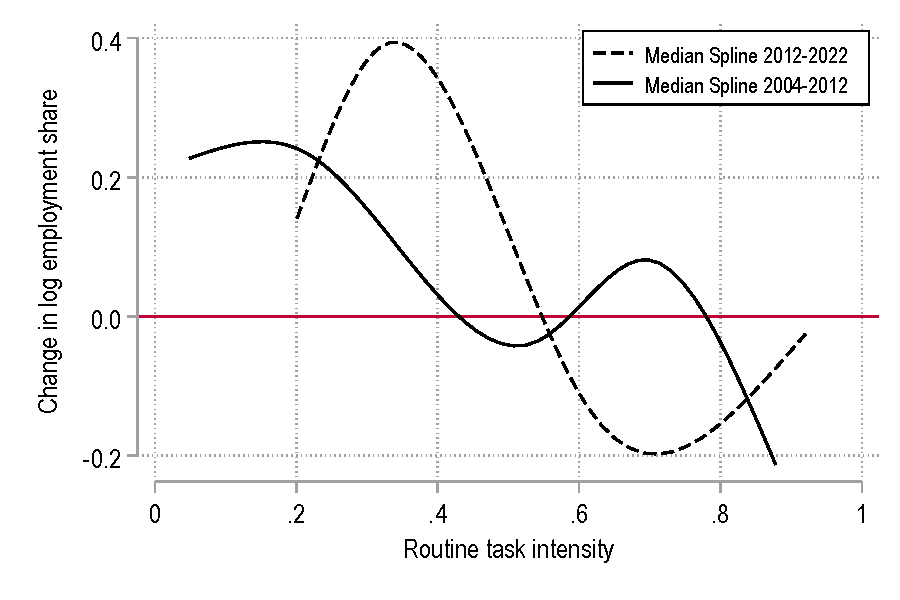
\includegraphics[width=0.75\textwidth]{figs/ch3/rti-employment.pdf}}
\par\end{centering}
\begin{centering}
\subfloat[\label{fig:Effect-of-RTI-onwage}Effect of RTI on Change in Log Real
Wages ]{\centering{}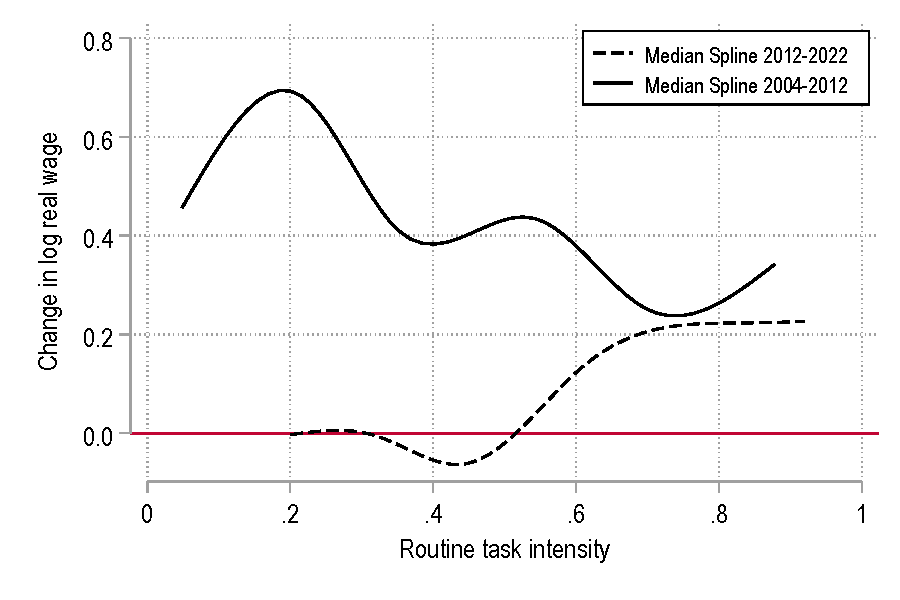
\includegraphics[width=0.75\textwidth]{figs/ch3/rti-wage.pdf}}
\par\end{centering}
\medskip{}

\textbf{Notes: }Point estimates from Graph \ref{fig:Smoothed-Changes-in-Wages-and-Employment-2}
calibrated with the occupation-specific routine task intensities from
O{*}NET data.
\end{figure}
\par\end{center}

\vspace{-1cm}

\subsubsection{Occupations' Role in Explaining Wage Polarization}

\begin{onehalfspace}
In order to identify the role of occupations in explaining wage differentials,
we followed the approach of \citet{2011Firpo,Fortin2016}. First,
we created a dataset consisting 9 deciles of wages for each occupation
for the years of 2004, 2012 and 2022, separately, $w_{jt}^{q}$for
$q$ = 10, 20, ... 90. Therefore, we created a dataset of 225 observations
for 25 occupation category and 9 deciles. \citet{Fortin2011} estimated
the following model to measure wage differences between years at wage
deciles:
\begin{eqnarray}
\Delta w_{j}^{q} & = & \widetilde{a_{j}}+\widetilde{b_{j}}w_{j0}^{q}+\lambda^{q}+\varepsilon_{j}^{q},\label{eq:simplelinearmodel}
\end{eqnarray}

Whereby, $w$ denotes wage, $j$ is occupation, $q$is the decile,
and $w_{0}$ stands for the base wage. The error term of the model
is the compound of decile-specific error component, $\lambda^{q}$,
which measures the change in return to unobservable skills\footnote{For example, if the unobservable skills in the regression, such as
the unmeasured school quality, changes in the returns to school quality
will be captured by the error component $\lambda^{q}$ if it is equally
distributed and rewarded across all occupations.}, and idiosyncratic error term, $\varepsilon_{j}^{q}$, which we assume
to be normally distributed. In this model, the parameter $\tilde{a_{j}}$
is the occupation-specific constant, and $\tilde{b_{j}}$ is the occupation-specific
slope. When the Eq. \ref{eq:simplelinearmodel} estimated, the intercept
$\tilde{a_{j}}$ captures between-occupation changes in wage dispersion
and $\tilde{b_{j}}$ captures the within-occupation changes. In the
second step of the analysis, they link the estimated intercepts and
slopes ($\tilde{a_{j}}$ and $\tilde{b_{j}}$) to the measures of
task content of occupations to analyze the effect of technology and
offshoring. Specifically, they used a task-occupation dataset to see
how well the task measures explains the intercepts and slopes.

In Figure \ref{fig:Changes-in-Real-Decile} we plot the real wage
changes of each period by using the raw data used in the estimation
in Table \ref{tab:reg fit of models-1} (N=255). The figure plots
the 255 observed wage changes as a function of the base wages. In
the first period, wage data yields a U-shaped pattern, which is well-known
in the related literature. In the second period, the curvature weakens.
The empirical strategy of the first stage analysis in Table \ref{tab:reg fit of models-1},
attempts to see the explanatory power of the simple linear model in
eq \ref{eq:simplelinearmodel} on explaining the variation reported
in Figure \ref{fig:Changes-in-Real-Decile}. Moreover, we report the
regression results to determine the exact value of the curvature in
Figure \ref{fig:Changes-in-Real-Decile} below:
\begin{eqnarray}
\widehat{\Delta wage} & = & \underset{(0.103)^{***}}{-0.978}logwage(2004)+\underset{(.019)^{***}}{.175}logwage(2004)^{2}+\underset{(0.135)^{***}}{1.548},\label{eq:quadeq}
\end{eqnarray}

The standard error values in this model indicate that the coefficients
are statistically significant at the 1\% significance level. Quadratic
form coefficient ($\pi_{2}$ in eq \ref{eq:quadratic}) implies that
there is a statistically significant convexity in the wage differences
in the period of 20004 to 2012.
\end{onehalfspace}
\begin{center}
\begin{figure}[H]
\caption{\label{fig:Changes-in-Real-Decile}Changes in Real Log Wages by Decile}

\begin{centering}
\subfloat[2004-2012]{
\centering{}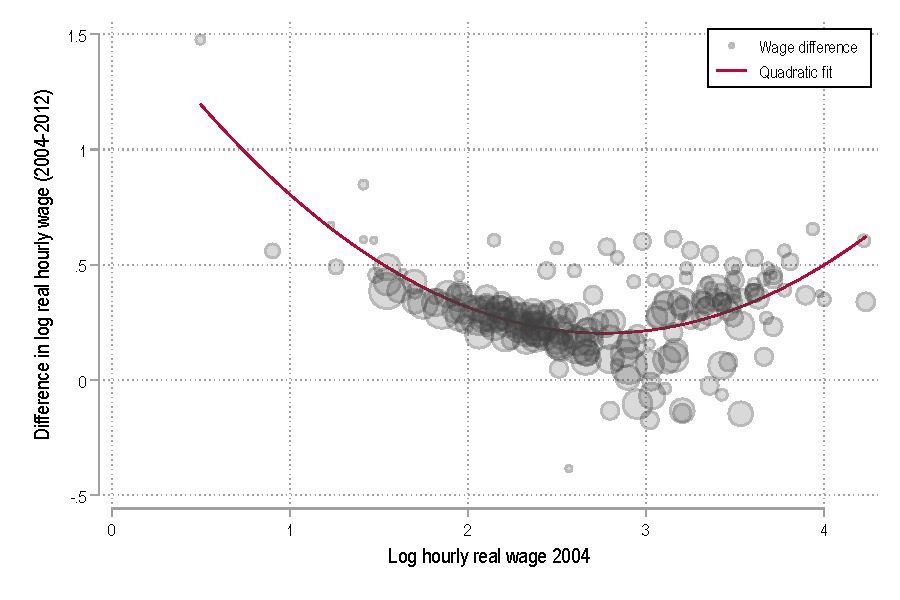
\includegraphics[width=1\textwidth]{figs/ch3/decile-wage-changes-2004-2012.pdf}}
\par\end{centering}
\begin{centering}
\subfloat[2012-2020]{
\centering{}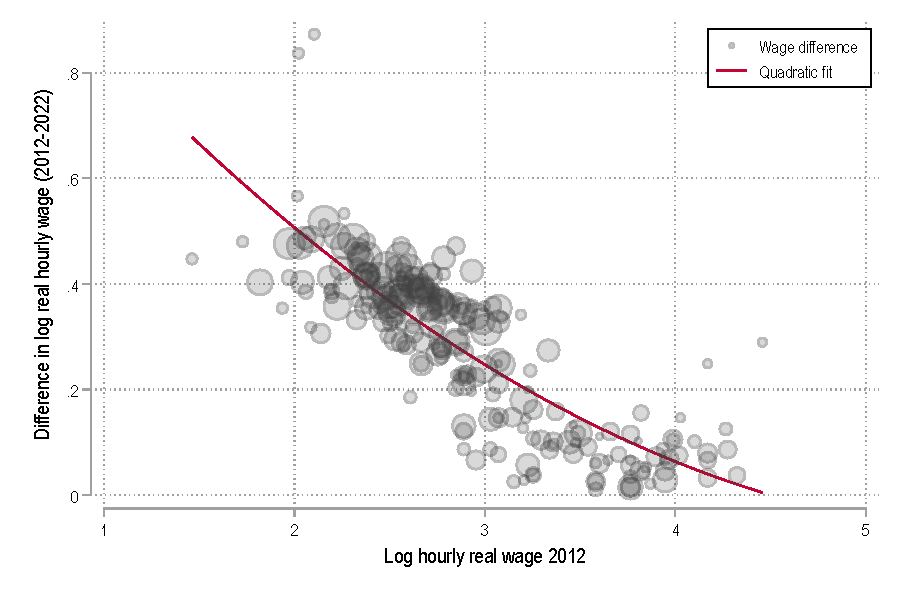
\includegraphics[width=1\textwidth]{figs/ch3/decile-wage-changes-2012-2022.pdf}}
\par\end{centering}
\medskip{}

\textbf{Notes: }Each point represents a decile for each occupation
and diameters are adjusted according to labor supply weight of each
plotted point.
\end{figure}
\par\end{center}

\vspace{-1cm}

\begin{onehalfspace}
Following \citet{2011Firpo}, we estimated several versions of Eq.
\ref{eq:simplelinearmodel}, which are reported in Table \ref{tab:reg fit of models-1}.
To evaluate the empirical performance of the models, we use two measures.
Firstly, the adjusted R-square values for each model are evaluated
to determine the extent to which the model performs in predicting
wages. However, due to the residual sampling error, \citet{2011Firpo}
denote that the wage change estimation does not explain all the variation
in the data.

The second measure of fit relies on the performance of each model
in explaining the curvature in Figure \ref{fig:Changes-in-Real-Decile}.
For each model, we run a quadratic regression of the residuals estimated
in the model on a linear and quadratic term in the base wage to see
the amount of decrease in the curvature, by using the following specification:
\begin{eqnarray}
\hat{\varepsilon_{j}^{q}} & = & \pi_{0}+\pi_{1}w_{j0}^{q}+\pi_{2}(w_{j0}^{q})^{2}+\upsilon_{j}^{q},\label{eq:quadratic}
\end{eqnarray}

As a reference, quadratic term coefficient ($\hat{\pi_{2}}$) from
the fitted regression of the raw data is 0.175 which is reported in
eq \ref{eq:quadeq}. In the first model of Table \ref{tab:reg fit of models-1}
(column 1), eq \ref{eq:simplelinearmodel} is estimated as a benchmark,
having only the base wage as an explanatory variable. Adjusted R-square
(0.027) shows that the explained variation in the data is negligible.
As expected, the linear model can not explain the curvature of the
changes in wages; thus, the curvature parameter in the residuals from
this model is close to \ref{eq:quadeq}.
\end{onehalfspace}
\begin{center}
\begin{table}[H]
\caption{\label{tab:reg fit of models-1}Regression Fit of Models for Changes
in Wages at Each Decile, by Two-Digit Occupation}

\begin{centering}
\noindent\resizebox{\textwidth}{!}{%
\begin{tabular}{>{\raggedright}p{4.5cm}r@{\extracolsep{0pt}.}lr@{\extracolsep{0pt}.}lr@{\extracolsep{0pt}.}lr@{\extracolsep{0pt}.}lr@{\extracolsep{0pt}.}lr@{\extracolsep{0pt}.}lr@{\extracolsep{0pt}.}l}
\toprule 
 & \multicolumn{2}{c}{(1)} & \multicolumn{2}{c}{(2)} & \multicolumn{2}{c}{(3)} & \multicolumn{2}{c}{(4)} & \multicolumn{2}{c}{(5)} & \multicolumn{2}{c}{(6)} & \multicolumn{2}{c}{(7)}\tabularnewline
\cmidrule{2-15} \cmidrule{4-15} \cmidrule{6-15} \cmidrule{8-15} \cmidrule{10-15} \cmidrule{12-15} \cmidrule{14-15} 
Occupation dummies & \multicolumn{2}{c}{} & \multicolumn{2}{c}{X} & \multicolumn{2}{c}{} & \multicolumn{2}{c}{X} & \multicolumn{2}{c}{X} & \multicolumn{2}{c}{X} & \multicolumn{2}{c}{X}\tabularnewline
Decile dummies & \multicolumn{2}{c}{} & \multicolumn{2}{c}{} & \multicolumn{2}{c}{X} & \multicolumn{2}{c}{X} & \multicolumn{2}{c}{X} & \multicolumn{2}{c}{} & \multicolumn{2}{c}{X}\tabularnewline
Base wage & \multicolumn{2}{c}{X} & \multicolumn{2}{c}{} & \multicolumn{2}{c}{} & \multicolumn{2}{c}{} & \multicolumn{2}{c}{X} & \multicolumn{2}{c}{X} & \multicolumn{2}{c}{X}\tabularnewline
Occupation{*}base wage (slope) & \multicolumn{2}{c}{} & \multicolumn{2}{c}{} & \multicolumn{2}{c}{} & \multicolumn{2}{c}{} & \multicolumn{2}{c}{X} & \multicolumn{2}{c}{X} & \multicolumn{2}{c}{}\tabularnewline
\cmidrule{2-15} \cmidrule{4-15} \cmidrule{6-15} \cmidrule{8-15} \cmidrule{10-15} \cmidrule{12-15} \cmidrule{14-15} 
Adj. $R^{2}$ & 0&027 & 0&420 & 0&108 & 0&560 & 0&821 & 0&808 & 0&601\tabularnewline
Curvature in resid. ($\beta_{2}$) & 0&193$^{***}$ & 0&120$^{***}$ & 0&186$^{***}$ & 0&113$^{***}$ & 0&0167 & 0&028$^{**}$ & 0&091$^{***}$\tabularnewline
(N=225) & (0&017) & (0&012) & (0&017) & (0&012) & (0&008) & (0&009) & (0&012)\tabularnewline
\bottomrule
\end{tabular}}
\par\end{centering}
\medskip{}

\textbf{Notes:} Regressions are estimated for each decile within each
occupation category. The independent variable is the wage changes
between years, represented as the difference between the logarithm
of wages for t $log(w_{t})$ and the logarithm of the wages at the
base year $log(w_{0})$. The analysis includes a total of 255 observations,
encompassing 25 occupations and 9 deciles for each occupation. To
account for the varying representation of occupations in the labor
market, the models are weighted by the labor supply allocated to each
occupation category in the base year, calculated as the product of
usual weekly working hours and the corresponding sampling weight for
each observation. Standard errors are in parentheses. {*}{*}{*} p<0.01;
{*}{*} p<0.05; {*}p<0.1. 
\end{table}

\par\end{center}

\vspace{-1cm}

\begin{onehalfspace}
If we only include the set of occupation dummies (the $\widetilde{a_{j}}'$s
) in the model, as in model 2, it explains 42\% of the raw variation
in the data. Model 2 also explains about a two third of the curvature,
which we see from the curvature parameter declining from 0.193 to
0.120, although it is still significant at the 1 percent significance
level. Since we did not include any other variable in Model 2, it
restricts of the same rate of increase in the wage deciles within
a given occupation category. This assumption relates to the case that
there is no within-occupation wage inequality. 

In model 3, we only include the decile dummies ($\lambda^{q}$'s).
The explanatory power of the model is too little (0.108), likewise
the residuals only explain a 3 percent of the curvature. This result
implies that the within-occupation change in wage inequality does
not explain the observed change in wages. In model 4, occupation dummies
and decile dummies are combined. The adjusted $R^{2}$ (0.560) indicates
that occupation-specific factors could explain the substantial portion
of within-occupation changes in the wage distribution. We can make
this inference by comparing the adjusted R-square values of model
4 and model 2. Since adding the decile dummies to Model 2 improves
the explanatory power only marginally, we can interpret this as the
increase in returns to skill has little impact on explaining variations
in wage levels within occupations. Thus, occupation-specific factors
has more effect on within-occupation wage dispersion.

The fit of the model improves substantially to 0.821 in Model 5, once
we introduced occupation-specific slopes ($\widetilde{b_{j}}$'s).
More importantly, the curvature parameter is no longer statistically
significant (0.0167). In other words, by using occupation-specific
slope, we can explain the wage polarization in the sample data. When
we compare the adjusted R-squared of Model 6 and Model 7, we see that
the occupation interactions have made significant impacted, rather
than decile dummies.

When contrasting the curvature between Model 2 and Model 7, considering
their minimal disparity, we can infer that the wage inequality observed
during the initial study period finds its primary explanation in the
occupation-specific variables. This observation underscores the significant
role played by these variables in clarifying the wage dynamics within
the studied period. Moreover, the result highlights the superiority
of individual-level task data from PIAAC in explaining wage dispersions,
rather than relying on occupation-level O{*}NET data.
\end{onehalfspace}
\begin{center}
\newpage
\par\end{center}
